%************************************************
\chapter{Basic Concepts}\label{ch:introductionplanning}
%************************************************
This chapter gives an introduction to the main concepts and notions in the context of planning for mobile robots as described in \cite{Choset_2005_5167}\cite{LaValle2006}.

The representation of the environment where a mobile robot is situated is called the \emph{workspace} or \emph{world}.
Typical representations of the workspace are either planar ($\mathbb{R}^2$), or three-dimensional($\mathbb{R}^3$), but also higher dimensional representation are possible.

Robots and obstacles can be described by geometric models using polygonal ($\mathbb{R}^2$), polyhedral ($\mathbb{R}^3$) or semi-algebraic sets \cite{LaValle2006}.

The \emph{configuration} of a robot is described by a set of parameters which enables the specification of the position of every point on the robot. The \emph{configuration space} of a robotic system is the space of all possible configurations.

  


\section{Classic Path Planning Problem}\label{sec:basic}
Statespace,
Configurationspace,
Obstacles in Configurationspace,
Workspace,
Actions,
Paths,
Trajectories,

\section{Constraints on Motion}\label{sec:model}
The 

Kinematic constraints are constraints on the velocities of a robot.


Holonomic:
A robot is called holonomic if all constraints can be expressed without using constraints on the velocity. 

A unicycle which can only move in one direction and is not allowed to change is orientation is also holonomic, since  it can be expressed without the use of derivates of state variables.
The formular is called a holonomic constraint.

Nonholonimc:
If state transitions can not be expressed without the use of velocities the system is called nonholonmic.
for example a robot with differential drive can roll forward and backward but not sideways. 
This no-slip constraint on the velocities of the vehicle is a nonholonimc constraint.
where velocities can not be removed by integration 

Therefore nonholonomic systems are sometimes referred to as nonintegrable systems (See Autonomouse Mobile Robots).


The following example of a nonholonomic robot taken from Priciples of Robot Motion is a robot with differential drive illustrated in Figure \ref{fig_diff}.
The configuration of the robot is determined by its position and orientation q(x,y,phi).
The left and the right wheel can be actuated by a motor given the speeds $u_l$ and $u_r$.
This yields the following system.

This can not be integrated to eliminate x and y, hence the system is nonholonomic (see Planning algorithms).
  
Dynamic constraints are constraints on the acceleration of the robot.  Typically accelerations limits are induced for examples by the torques that are applied to motors, which results in minimal and maximal acceleration bounds.


\section{Representation of the Environment}\label{sec:representation}
Fixed Cell Decomposition
Exact Cell Decomposition
Approximate Cell Decomposition
Visibility Graph
Voronoi Regions

\section{Planning}\label{sec:global}
Global Planning:
Breadth-First Search (BFS)
Depth-First Search (DFS)
Dijkstra's and A* algorithm
An illustration is given in Figure~\ref{fig:fig_overview}
\begin{figure}[thpb]
	  \myfloatalign
      \footnotesize
      \centering
    \subfloat[Dijkstra algorithm]
    {  \label{fig:fig_djikstra}
        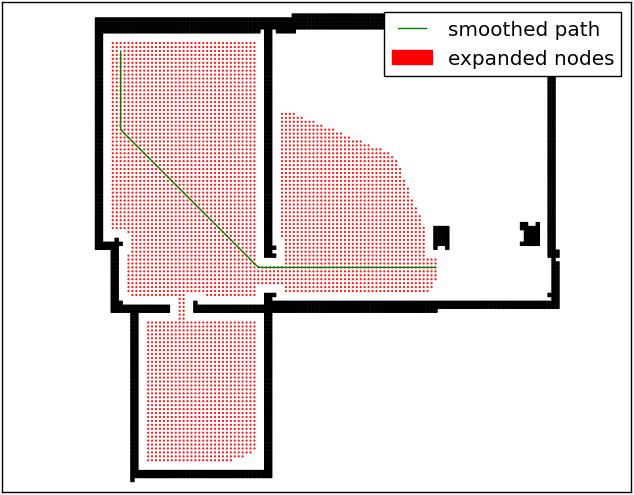
\includegraphics[width=0.75\textwidth]{figures/fig_djikstra.png}
        %\caption{Dijkstra}
    }
    
    \subfloat[A* algorithm]
    {  \label{fig:fig_astar}
       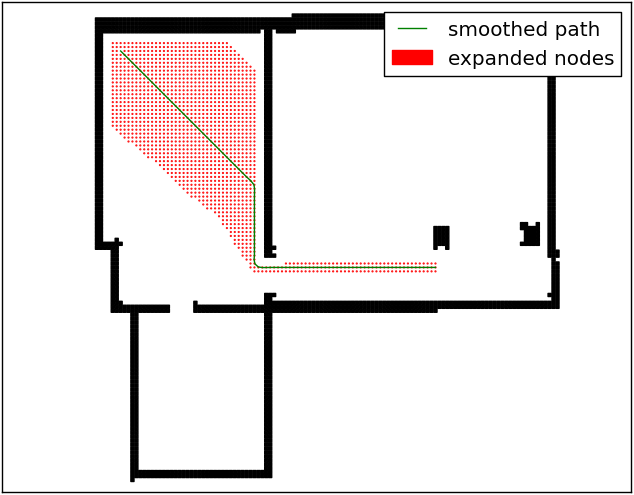
\includegraphics[width=0.75\textwidth]{figures/fig_astar.png}
       %\caption{A*}
    }
   \caption[Djikstra's and A* algorithm.]{The difference between Djikstra's and A* algorithm searching for a shortest path in a grid representation of a building. A* is more effective, as it visits by far less nodes in the search graph. }
\label{fig:fig_overview}
\end{figure}
Examples: 
Rapidly Exploring Randomized Trees (RRT)
Probabilistic Road Maps (PRM)
Potential Field
Meta-Heuristic approaches

Local Planning:
The next chapter investigates local planning methods.

%*****************************************
%*****************************************
%*****************************************
%*****************************************
%*****************************************




